\documentclass[tikz,border=2mm]{standalone}
\usepackage{amsmath}
\usepackage{amssymb}
\usetikzlibrary{shapes,arrows,positioning,calc,patterns,decorations.pathreplacing,shadows,fit,backgrounds}

\definecolor{wacvblue}{rgb}{0.21,0.49,0.74}
\definecolor{minorityred}{RGB}{220,50,47}
\definecolor{highlightgreen}{RGB}{56,142,60}
\definecolor{highlightgray}{RGB}{128,128,128}
\definecolor{purpleaccent}{RGB}{123,31,162}
\definecolor{orangeaccent}{RGB}{255,165,0}

\begin{document}

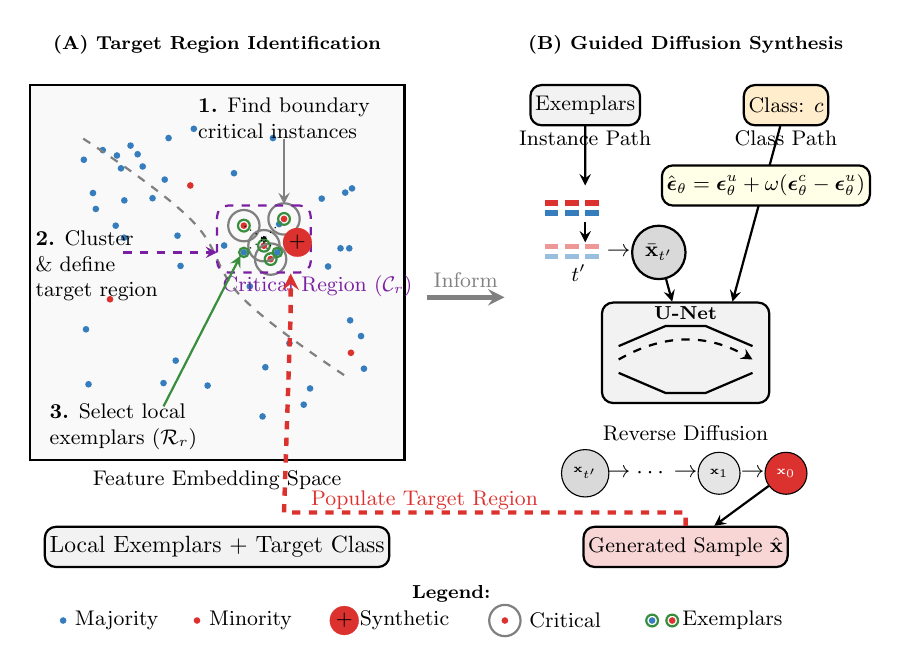
\begin{tikzpicture}[scale=0.85, every node/.style={scale=0.85},
    datapoint/.style={circle,inner sep=1pt},
    majority/.style={datapoint,fill=wacvblue},
    minority/.style={datapoint,fill=minorityred},
    boundary/.style={thick,dashed,gray},
    highlight/.style={circle,draw=highlightgray,thick,minimum size=6pt},
    region/.style={draw=purpleaccent,thick,dashed,rounded corners},
    arrow/.style={->,>=stealth,thick},
    block/.style={rectangle,draw,thick,rounded corners,minimum height=6mm,inner sep=2pt},
    label/.style={font=\small},
    title/.style={font=\footnotesize\bfseries}
]

% Panel A: Target Region Identification
\begin{scope}[local bounding box=panelA]
    % Title
    \node[title] at (0,3.4) {(A) Target Region Identification};
    
    % Feature embedding space
    \begin{scope}[shift={(0,0)}]
        % Background
        \fill[gray!5] (-2.8,-2.8) rectangle (2.8,2.8);
        \draw[thick] (-2.8,-2.8) rectangle (2.8,2.8);
        \node[label] at (0,-3.1) {Feature Embedding Space};
        
        % Majority class points
        \foreach \i in {1,...,30} {
            \pgfmathsetmacro{\x}{rand*2.2}
            \pgfmathsetmacro{\y}{rand*2.2}
            \node[majority] at (\x,\y) {};
        }
        
        % More concentrated majority cluster
        \foreach \i in {1,...,12} {
            \pgfmathsetmacro{\x}{-1.2+rand*0.7}
            \pgfmathsetmacro{\y}{1.2+rand*0.7}
            \node[majority] at (\x,\y) {};
        }
        
        % Minority class points (sparse)
        \node[minority] (m1) at (0.4,0.7) {};
        \node[minority] (m2) at (0.7,0.4) {};
        \node[minority] (m3) at (1.0,0.8) {};
        \node[minority] (m4) at (-0.4,1.3) {};
        \node[minority] (m5) at (2.0,-1.2) {};
        \node[minority] (m6) at (-1.6,-0.4) {};
        \node[minority] (m7) at (0.8,0.2) {};
        
        % Decision boundary
        \draw[boundary] plot[smooth,tension=0.7] coordinates {(-2.0,2.0) (-0.4,0.8) (0.4,-0.4) (2.0,-1.6)};
        
        % Step 1: Highlight boundary-critical points
        \node[highlight,fit=(m1)] {};
        \node[highlight,fit=(m2)] {};
        \node[highlight,fit=(m3)] {};
        \node[highlight,fit=(m7)] {};
        
        % Step 1 annotation
        \draw[arrow,highlightgray] (1.0,2.0) -- (1.0,1.02);
        \node[label,align=left] at (1.0,2.3) {\textbf{1.} Find boundary\\critical instances};
        
        % Step 2: Cluster region
        \node[region,minimum width=1.4cm,minimum height=1cm] (criticalregion) at (0.7,0.5) {};
        \node[label,purpleaccent] at (1.5,-0.2) {Critical Region ($\mathcal{C}_r$)};
        
        % Step 2 annotation
        \node[label,align=left] at (-1.8,0.1) {\textbf{2.} Cluster \\ \& define\\target region};
        \draw[arrow,purpleaccent,dashed] (-1.4,0.3) -- (0.0,0.3);
        
        % Step 3: Centroid and local exemplars
        \node[draw,fill=black,star,star points=4,inner sep=0.5pt] (centroid) at (0.7,0.5) {};
        
        % Local exemplars (both classes)
        \foreach \point in {(0.4,0.7), (0.7,0.4), (1.0,0.8), (0.8,0.2)} {
            \draw[dotted,thin] (centroid) -- \point;
            \draw[highlightgreen,thick] \point circle (2.5pt);
        }
        % Also select some majority points as exemplars
        \node[majority] (e1) at (0.4,0.3) {};
        \node[majority] (e2) at (0.9,0.3) {};
        \draw[dotted,thin] (centroid) -- (e1);
        \draw[dotted,thin] (centroid) -- (e2);
        \draw[highlightgreen,thick] (e1) circle (2pt);
        \draw[highlightgreen,thick] (e2) circle (2pt);
        
        % Step 3 annotation
        \node[label,align=left] at (-1.4,-2.3) {\textbf{3.} Select local\\exemplars ($\mathcal{R}_r$)};
        \draw[arrow,highlightgreen] (-0.8,-2.0) -- (0.35,0.25);
    \end{scope}
    
    % Output box
    \node[block,fill=gray!10] (outputA) at (0,-4.1) {Local Exemplars + Target Class};
\end{scope}

% Panel B: Instance and Class-Guided Diffusion Synthesis
\begin{scope}[xshift=7cm,local bounding box=panelB]
    % Title
    \node[title] at (0,3.4) {(B) Guided Diffusion Synthesis};
    
    % Input representations
    \node[block,fill=gray!10] (exemplars) at (-1.5,2.5) {\small Exemplars};
    \node[block,fill=orangeaccent!20] (targetclass) at (1.5,2.5) {\small Class: $c$};
    
    % Instance conditioning path
    \node[label] at (-1.5,2.0) {Instance Path};
    \draw[arrow] (exemplars) -- (-1.5,1.3);
    
    % Show partial diffusion process
    \begin{scope}[shift={(-1.5,0.6)}]
        % Original exemplars
        \foreach \i in {0,1,2} {
            \fill[minorityred] (-0.6+\i*0.3,0.4) rectangle ++(0.2,0.08);
            \fill[wacvblue] (-0.6+\i*0.3,0.25) rectangle ++(0.2,0.08);
        }
        % Arrow down
        \draw[arrow] (0,0.15) -- (0,-0.15);
        % Noised versions
        \foreach \i in {0,1,2} {
            \fill[minorityred!50] (-0.6+\i*0.3,-0.25) rectangle ++(0.2,0.08);
            \fill[wacvblue!50] (-0.6+\i*0.3,-0.4) rectangle ++(0.2,0.08);
        }
        % Aggregation
        \node at (0.5,-0.3) {$\rightarrow$};
        \node[draw,thick,circle,fill=gray!30,minimum size=5mm] (aggregated) at (1.1,-0.3) {\small $\bar{\mathbf{x}}_{t'}$};
    \end{scope}
    
    % Class conditioning path
    \node[label] at (1.5,2.0) {Class Path};
    
    % U-Net architecture (simplified)
    \node[block,minimum width=2.5cm,minimum height=1.5cm,fill=gray!10] (unet) at (0,-1.2) {};
    \node[title] at (0,-0.6) {U-Net};
    
    % U-Net internal structure
    \begin{scope}[shift={(0,-1)}]
        \draw[thick] (-1.0,-0.5) -- (-0.3,-0.8) -- (0.3,-0.8) -- (1.0,-0.5);
        \draw[thick] (-1.0,-0.1) -- (-0.3,0.2) -- (0.3,0.2) -- (1.0,-0.1);
        \draw[arrow,dashed] (-1.0,-0.3) to[out=30,in=150] (1.0,-0.3);
    \end{scope}   
    % Inputs to U-Net
    \draw[arrow] (targetclass) -- ($(unet.north)+(0.7,0)$);
    \draw[arrow] (aggregated) -- ($(unet.north)+(-0.2,0.0)$);
    \node[label] at (-1.6,-0.01) {$t'$};
    
    % Classifier-free guidance formula
    \node[block,fill=yellow!10,font=\small] at (1.2,1.3) {$\hat{\boldsymbol{\epsilon}}_\theta = \boldsymbol{\epsilon}_\theta^u + \omega(\boldsymbol{\epsilon}_\theta^c - \boldsymbol{\epsilon}_\theta^u)$};
    
    % Reverse diffusion chain
    \node[label] at (0,-2.4) {Reverse Diffusion};
    \begin{scope}[shift={(0,-3.0)}]
        \node[draw,circle,fill=gray!30,minimum size=4mm] (xt) at (-1.5,0) {\tiny $\mathbf{x}_{t'}$};
        \node at (-1.0,0) {$\rightarrow$};
        \node at (-0.5,0) {$\cdots$};
        \node at (0,0) {$\rightarrow$};
        \node[draw,circle,fill=gray!20,minimum size=4mm] at (0.5,0) {\tiny $\mathbf{x}_1$};
        \node at (1.0,0) {$\rightarrow$};
        \node[draw,circle,fill=minorityred,text=white,minimum size=4mm] (x0) at (1.5,0) {\tiny $\mathbf{x}_0$};
    \end{scope}
    
    % Generated sample
    \node[block,fill=minorityred!20] (generated) at (0,-4.1) {\small Generated Sample $\hat{\mathbf{x}}$};
    \draw[arrow] (x0) -- (generated);
\end{scope}

% NOW draw the arrow between panels (after both are defined)
\draw[arrow,ultra thick,gray] ($(panelA.east)+(0.1,0)$) -- node[above,label] {Inform} ($(panelB.west)+(-0.1,0)$);

% Feedback arrow
\draw[arrow,ultra thick,minorityred,dashed] 
    (generated.north) -- ++(0,0.2) -- ++(-6.0,0) -- ++(0.1,3.0) 
    to[out=90,in=270] ($(criticalregion.south)+(0.4,0)$);
\node[label,minorityred] at (3.1,-3.4) {Populate Target Region};

% Add a new synthetic point in the critical region
\node[minority,draw=minorityred,line width=0.01pt] at (1.2,0.45) {\small +};

% Legend
\begin{scope}[shift={(2.5,-5.2)}]
    \node[title] at (1,0.4) {Legend:};
    \node[majority] at (-4.8,0) {};
    \node[label] at (-4.0,0) {Majority};
    \node[minority] at (-2.8,0) {};
    \node[label] at (-2.0,0) {Minority};
    \node[minority,draw=minorityred,line width=0.1pt] at (-0.6,0) {\small +};
    \node[label] at (0.3,0) {Synthetic};
    % Critical instances
    \node[minority] (m8) at (1.8,0) {};
    \node[highlight,fit=(m8)] {};
    \node[label] at (2.7,0) {Critical};
    % Selected exemplars
    \node[majority] (m9) at (4.0,0) {};
    \draw[highlightgreen,thick] (4.0,0) circle (2.5pt);
    \node[minority] (m10) at (4.3,0) {};
    \draw[highlightgreen,thick] (4.3,0) circle (2.5pt);
    \node[label] at (5.2,0) {Exemplars}; 
\end{scope}

\end{tikzpicture}

\end{document} 